\documentclass[tikz,border=4pt]{standalone}
\usepackage[T1]{fontenc}
\usepackage{mathptmx}
\usetikzlibrary{arrows.meta,calc}
\begin{document}
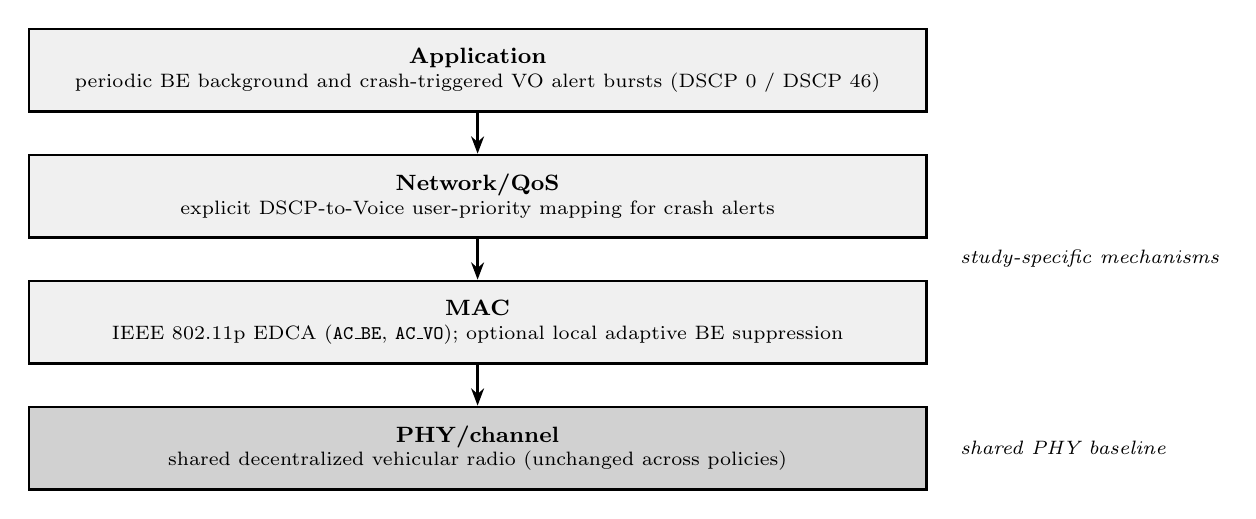
\begin{tikzpicture}[
  font=\footnotesize,
  >=Stealth,
  thick,
  box/.style={draw, thick, align=center, inner sep=6pt, minimum width=11.4cm},
  layer/.style={box, fill=black!6, minimum height=1.05cm},
  phy/.style={box, fill=black!18, minimum height=1.05cm},
  lbl/.style={font=\scriptsize\itshape, align=center},
  arr/.style={-{Stealth[length=2.2mm]}, thick},
]
  \node[layer] (app) at (0,4.80) {%
    \textbf{Application}\\[-1pt]
    {\scriptsize periodic BE background and crash-triggered VO alert bursts (DSCP~0~/~DSCP~46)}};
  \node[layer] (net) at (0,3.20) {%
    \textbf{Network/QoS}\\[-1pt]
    {\scriptsize explicit DSCP-to-Voice user-priority mapping for crash alerts}};
  \node[layer] (mac) at (0,1.60) {%
    \textbf{MAC}\\[-1pt]
    {\scriptsize IEEE~802.11p EDCA (\texttt{AC\_BE}, \texttt{AC\_VO}); optional local adaptive BE suppression}};
  \node[phy]  (phy) at (0,0.00) {%
    \textbf{PHY/channel}\\[-1pt]
    {\scriptsize shared decentralized vehicular radio (unchanged across policies)}};

  \draw[arr] (app.south) -- (net.north);
  \draw[arr] (net.south) -- (mac.north);
  \draw[arr] (mac.south) -- (phy.north);

  \node[lbl, anchor=west] at (6.00,2.40)
    {study-specific mechanisms};
  \node[lbl, anchor=west] at (6.00,0.00)
    {shared PHY baseline};
\end{tikzpicture}
\end{document}
